\setcolumnwidth{38mm, 132mm}
\setlength{\columnsep}{10mm}

\begin{paracol}{2}
\switchcolumn[1]
\noindent{\color{stewartblue}\textsf{\textbf{VÍ DỤ 2}}}\quad Nếu một thanh hoặc một đoạn dây kim loại là đồng chất, thì \textit{khối lượng riêng tuyến tính} của nó là đều và được định nghĩa là khối lượng trên một đơn vị chiều dài ($\rho = m/l$), đo bằng kilôgam trên mét. Tuy nhiên, giả sử rằng thanh không đồng chất nhưng khối lượng của nó tính từ đầu bên trái đến điểm $x$ là $m = f(x)$, như minh họa trong Hình~5.

\switchcolumn*
\switchcolumn[0]
\vspace*{1.2em}
\noindent\textbf{\textsf{HÌNH 5}}

\switchcolumn[1]
\begin{center}
  \vspace{-0.8em}
  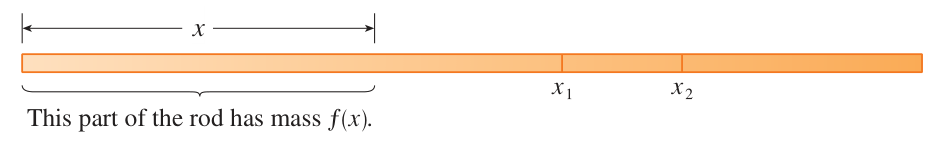
\includegraphics[width=\linewidth]{images/p0263_fig1.png}
  \vspace{-0.4em}
\end{center}

Khối lượng của phần thanh nằm giữa $x = x_1$ và $x = x_2$ được cho bởi $\Delta m = f(x_2) - f(x_1)$, do đó khối lượng riêng trung bình của phần thanh đó là
\begin{equation*}
  \text{khối lượng riêng trung bình} = \frac{\Delta m}{\Delta x} = \frac{f(x_2) - f(x_1)}{x_2 - x_1}
\end{equation*}

Nếu bây giờ ta cho $\Delta x \to 0$ (nghĩa là $x_2 \to x_1$), ta đang tính khối lượng riêng trung bình trên các khoảng ngày càng nhỏ hơn. \textbf{Khối lượng riêng tuyến tính} $\rho$ tại $x_1$ là giới hạn của các khối lượng riêng trung bình này khi $\Delta x \to 0$; tức là, khối lượng riêng tuyến tính là tốc độ biến thiên của khối lượng theo chiều dài. Dưới dạng ký hiệu,
\begin{equation*}
  \rho = \lim_{\Delta x \to 0} \frac{\Delta m}{\Delta x} = \frac{dm}{dx}
\end{equation*}

Như vậy, khối lượng riêng tuyến tính của thanh là đạo hàm của khối lượng theo chiều dài.
\par
Chẳng hạn, nếu $m = f(x) = \sqrt{x}$, trong đó $x$ được đo bằng mét và $m$ đo bằng kilôgam, thì khối lượng riêng trung bình của phần thanh ứng với $1 \le x \le 1{,}2$ là
\begin{equation*}
  \frac{\Delta m}{\Delta x} = \frac{f(1{,}2) - f(1)}{1{,}2 - 1} = \frac{\sqrt{1{,}2} - 1}{0{,}2} \approx 0{,}48\text{ kg/m}
\end{equation*}
trong khi khối lượng riêng ngay tại $x = 1$ là
\begin{equation*}
  \rho = \left.\frac{dm}{dx}\right|_{x=1} = \left.\frac{1}{2\sqrt{x}}\right|_{x=1} = 0{,}50\text{ kg/m} \qquad {\color{stewartblue}\blacksquare}
\end{equation*}

\vspace{1em}

\switchcolumn*
\switchcolumn[0]
\vspace*{0.2em}
\noindent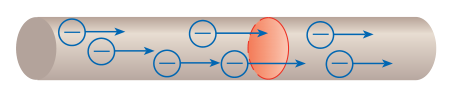
\includegraphics[width=\linewidth]{images/p0263_fig2.png}\\[4pt]
\textbf{\textsf{HÌNH 6}}

\switchcolumn[1]
\noindent{\color{stewartblue}\textsf{\textbf{VÍ DỤ 3}}}\quad Dòng điện xuất hiện bất cứ khi nào các điện tích chuyển động. Hình~6 minh họa một phần của dây dẫn và các electron chuyển động qua một tiết diện phẳng, được tô màu đỏ. Nếu $\Delta Q$ là điện lượng thuần đi qua tiết diện này trong một khoảng thời gian $\Delta t$, thì dòng điện trung bình trong khoảng thời gian này được định nghĩa là
\begin{equation*}
  \text{dòng điện trung bình} = \frac{\Delta Q}{\Delta t} = \frac{Q_2 - Q_1}{t_2 - t_1}
\end{equation*}

Nếu ta lấy giới hạn của dòng điện trung bình này trên các khoảng thời gian ngày càng nhỏ hơn, ta nhận được đại lượng gọi là \textbf{dòng điện} $I$ tại một thời điểm $t_1$ cho trước:
\begin{equation*}
  I = \lim_{\Delta t \to 0} \frac{\Delta Q}{\Delta t} = \frac{dQ}{dt}
\end{equation*}

Như vậy, dòng điện là tốc độ dòng điện tích chảy qua một bề mặt. Nó được đo bằng đơn vị điện tích trên một đơn vị thời gian (thường là culông trên giây, gọi là ampe). \hfill {\color{stewartblue}\blacksquare}

\end{paracol}
